%%%%%%%%%%%%%%%%%%%%%%%%%%%%%%%%%%%%%%%%%%%%%%%%%%%%%%%%%%%%%%%%%%%%%%%
% Created on Mon June 5, 2023
% @author: Giselle Labrador Badia (@gisslab)
%
% This report analyses OB auction files for early covid period. 
% It is based on the code files auction_prices_analysis.py, 
% auction_prices_timeseries_plots, fed_mbs
%%%%%%%%%%%%%%%%%%%%%%%%%%%%%%%%%%%%%%%%%%%%%%%%%%%%%%%%%%%%%%%%%%%%%%%




\documentclass[11pt,a4paper]{article}


\usepackage[utf8]{inputenc}
\usepackage[spanish,english]{babel}
\usepackage{apacite}
\usepackage[round]{natbib}
\usepackage{hyperref}
\bibliographystyle{apacite}


\usepackage[margin = 1in, top=1.5cm,bottom=1.5cm]{geometry}% Margins
\setlength{\parindent}{2em}
\setlength{\parskip}{0.3em}
\usepackage{setspace} % Setting the spacing between lines
\usepackage{hyperref} % To create hyperlinks within the document
\spacing{1.15}

%images
\usepackage{graphicx}
% \usepackage{subcaption}
\usepackage{caption}
% subcaption was interfering with the figure count, fix below
\usepackage{subcaption, xparse}

\usepackage[capposition=top]{floatrow}
\captionsetup[sub]{font=footnotesize,labelfont={bf,sf}}

\begin{document}

\title{Analysis of Auctions in OB in the Early Covid Period}

\maketitle



\section{FED purchases of MBS}

\begin{figure}[h]
    \centering
    \begin{subfigure}[b]{0.49\textwidth}
      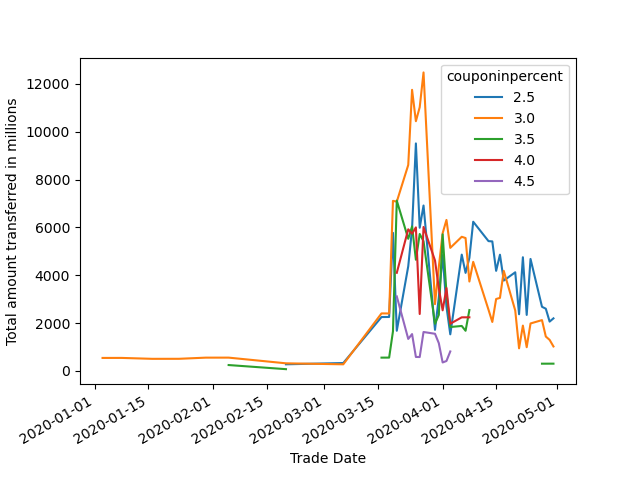
\includegraphics[width=0.998\textwidth]{../results/figures/FNMA_daily_purchases_tradedate_amount.png}
      \caption{ Quantity by trade date}
     \end{subfigure}
     \begin{subfigure}[b]{0.49\textwidth}
      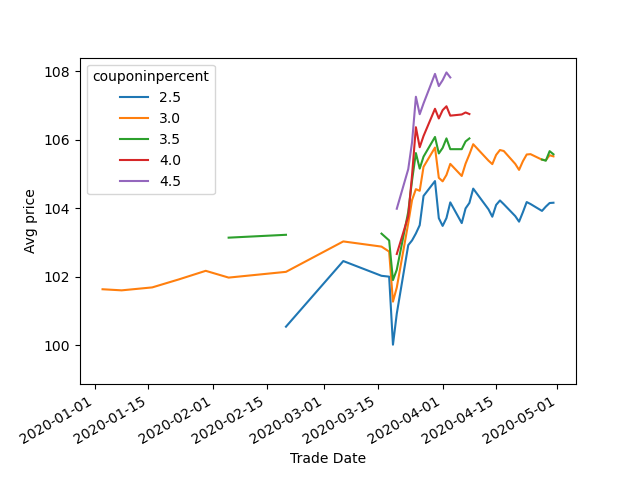
\includegraphics[width=0.998\textwidth]{../results/figures/FNMA_daily_purchases_tradedate_price.png}
      \caption{ Price by trade date}
     \end{subfigure}
    \begin{subfigure}[b]{0.49\textwidth}
        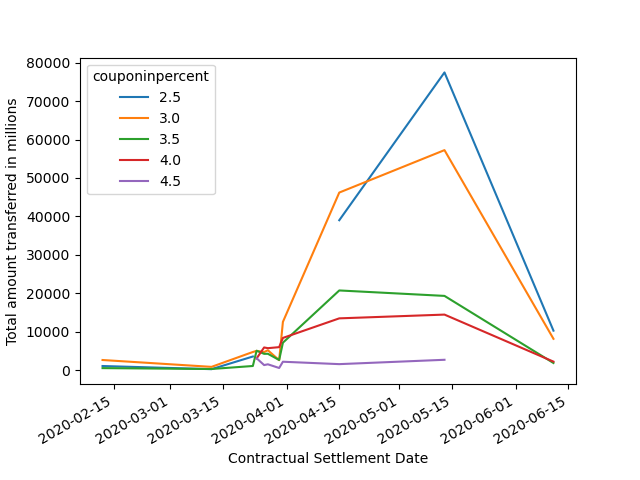
\includegraphics[width=0.998\textwidth]{../results/figures/FNMA_daily_purchases_contractualsettlementdate_amount.png}
        \caption{ Quantity by settlement date}
       \end{subfigure}
       \begin{subfigure}[b]{0.49\textwidth}
        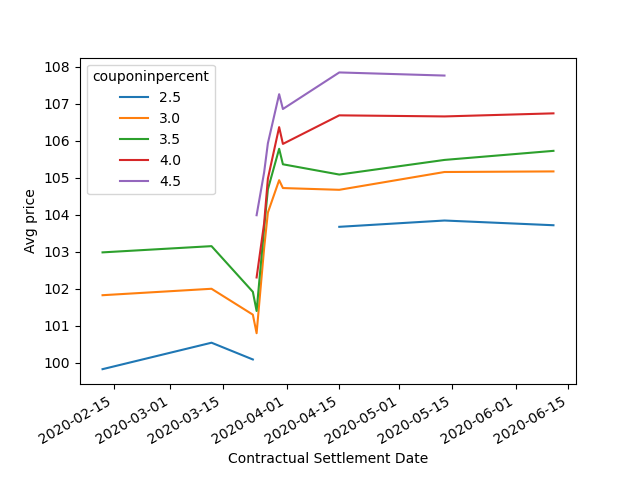
\includegraphics[width=0.998\textwidth]{../results/figures/FNMA_daily_purchases_contractualsettlementdate_price.png}
        \caption{ Price by settlement date}
       \end{subfigure}
     \caption{FED purchases of FNMA products in the early COVID period} 
     \begin{minipage}{\textwidth}
        \footnotesize{\textit{Notes:} The figure shows the daily time series of amounts and  prices of FED purchases of FNMA products and 30 year maturity. Colors represent different coupons. } 
        \end{minipage}
\end{figure}

\pagebreak
\section{OB Auctions in the Early Covid Period}

The following figures shows OB auctions mean, median higher bid, quantities and number of auctions that occured daily from January 1st to April 30th 2020.

\begin{figure}[h]
  \centering
  \begin{subfigure}[b]{0.49\textwidth}
      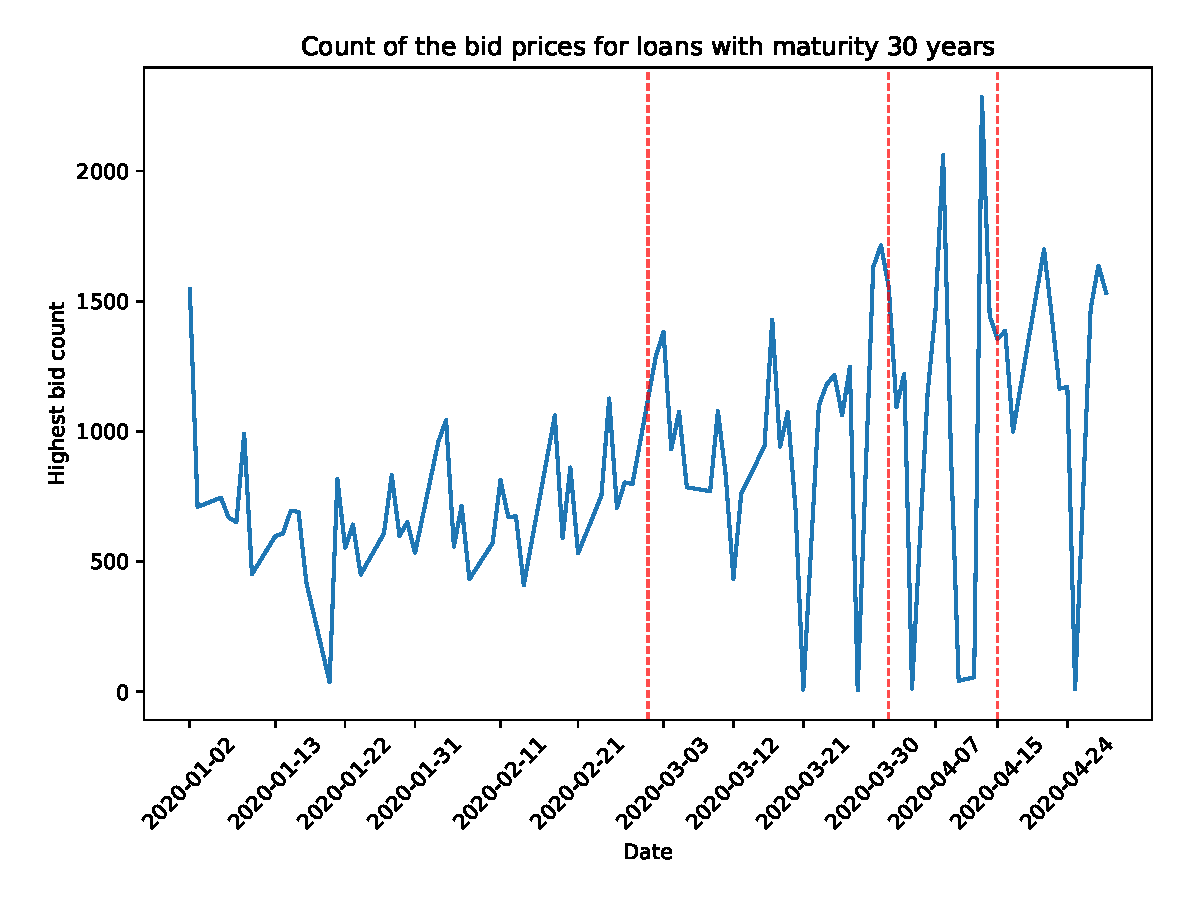
\includegraphics[width=0.998\textwidth]{../results/figures/winner_bid_count_mat30_loan1_timeseries_nr_1_7.pdf}
      \caption{ Number of auctions}
     \end{subfigure}
     \begin{subfigure}[b]{0.49\textwidth}
      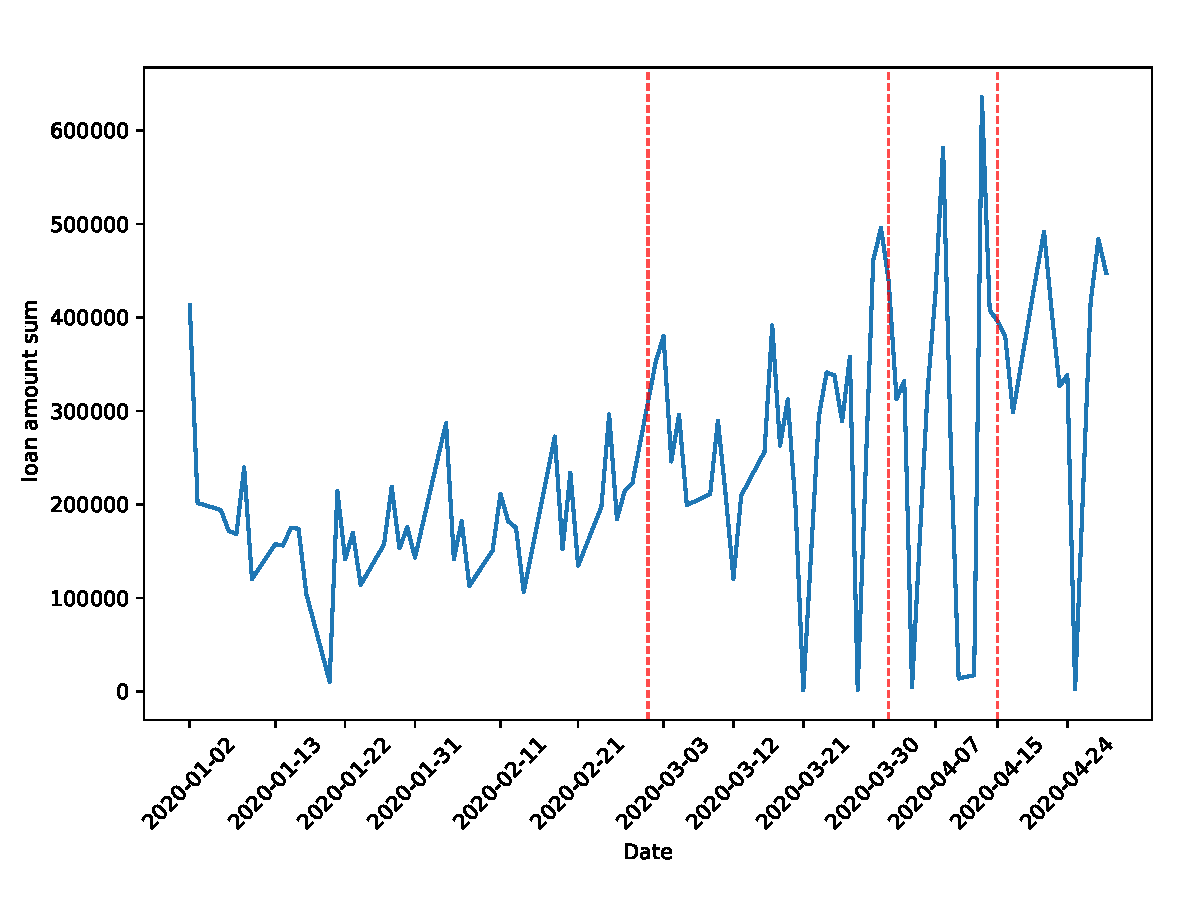
\includegraphics[width=0.998\textwidth]{../results/figures/LoanAmount_sum_mat30_loan1_timeseries_nr_1_7.pdf}
      \caption{ Daily loan amount}
     \end{subfigure}
     \begin{subfigure}[b]{0.49\textwidth}
      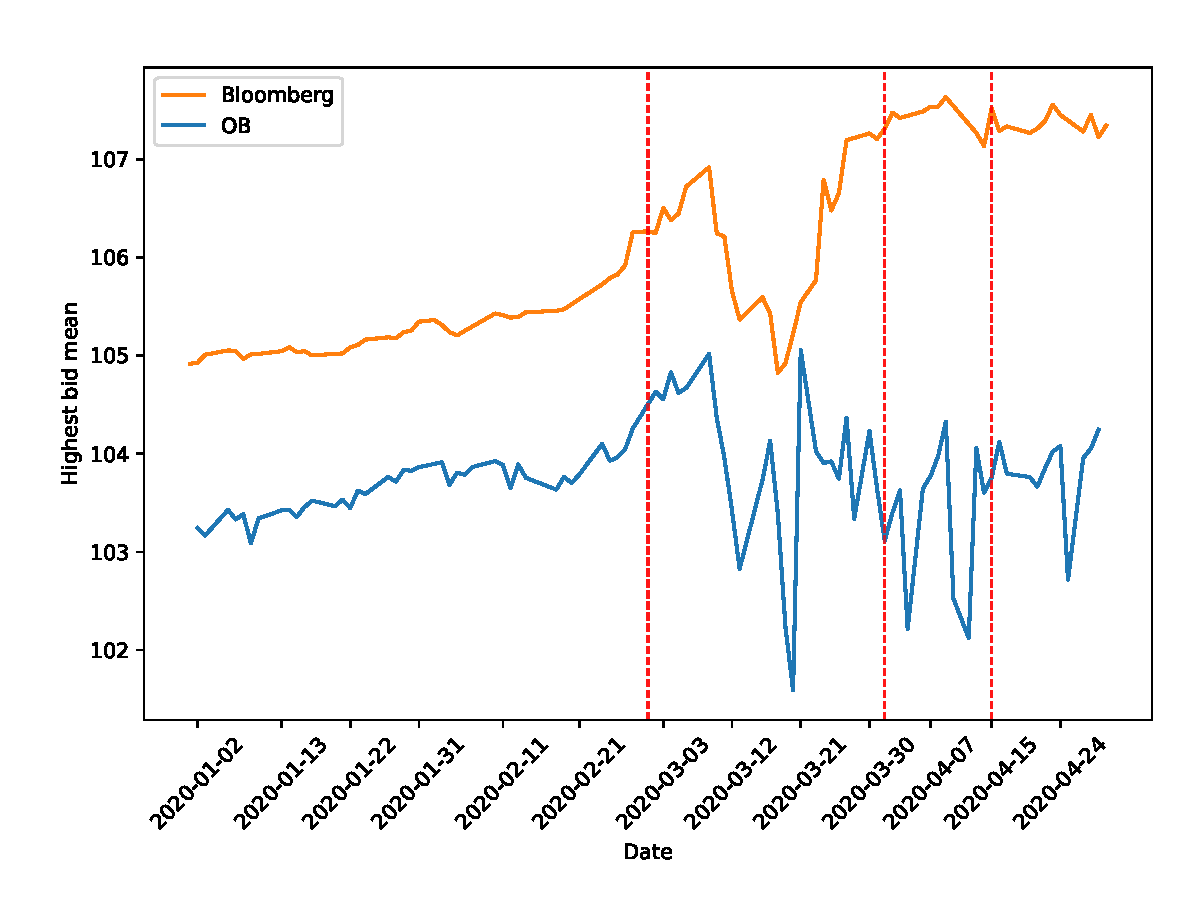
\includegraphics[width=0.998\textwidth]{../results/figures/w_winner_bid_mean_mat30_loan1_timeseries_nr_1_7.pdf}
      \caption{ Weighted mean of highest bid}
     \end{subfigure}
     \begin{subfigure}[b]{0.49\textwidth}
      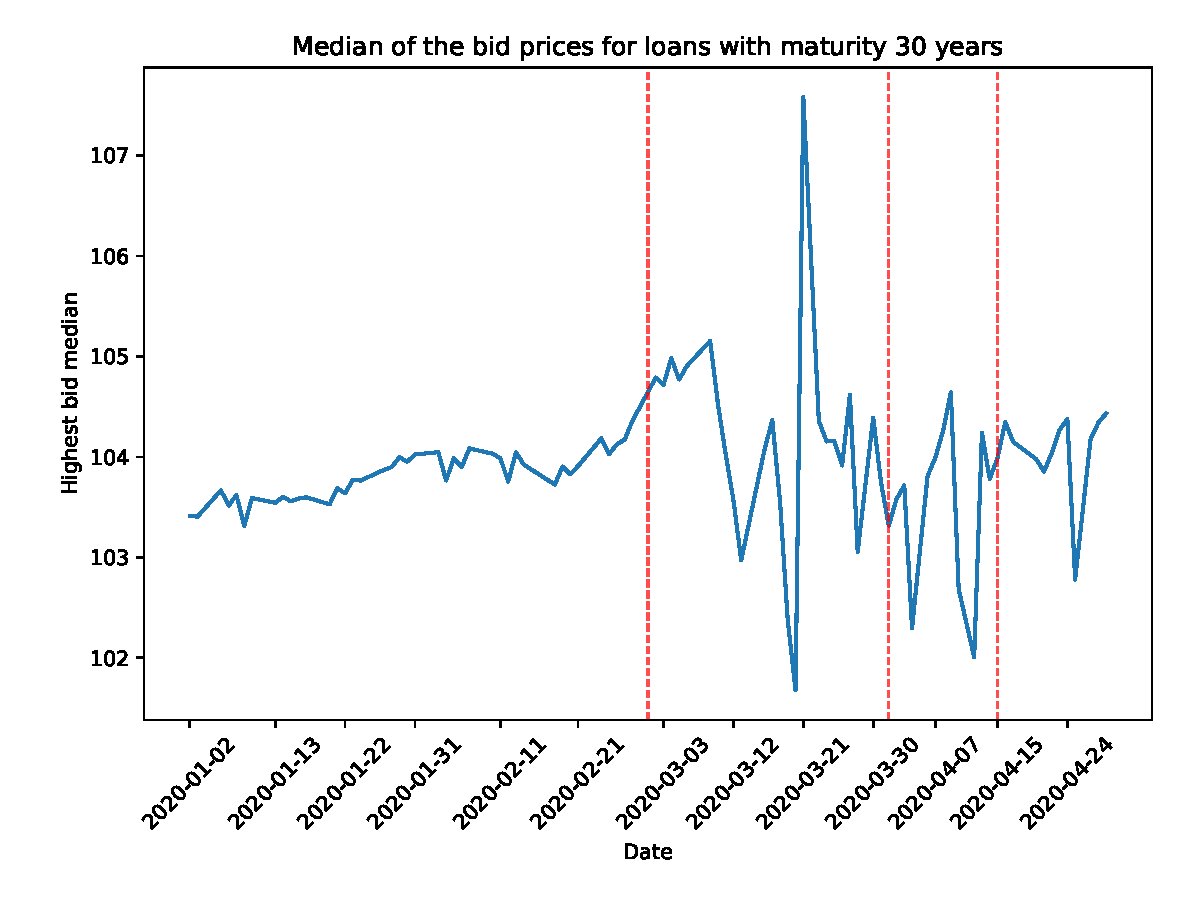
\includegraphics[width=0.998\textwidth]{../results/figures/winner_bid_median_mat30_loan1_timeseries_nr_1_7.pdf}
      \caption{ Median of highest bid}
     \end{subfigure}
   \caption{FED purchases of FNMA products in the early COVID period} 
   \begin{minipage}{\textwidth}
      \footnotesize{\textit{Notes:} The figure shows the daily time series of auctios for Conforming loans 30 year maturity. The vertical lines are March 1, April 1st and April 15th. For reference, Bloomberg TBA prices are aggregated for all forward months and coupons between 1 and 7. }
      \end{minipage}
\end{figure}

\pagebreak
\subsection{Comparison of note rates}

\begin{figure}[h]
  \centering
  \begin{subfigure}[b]{0.49\textwidth}
      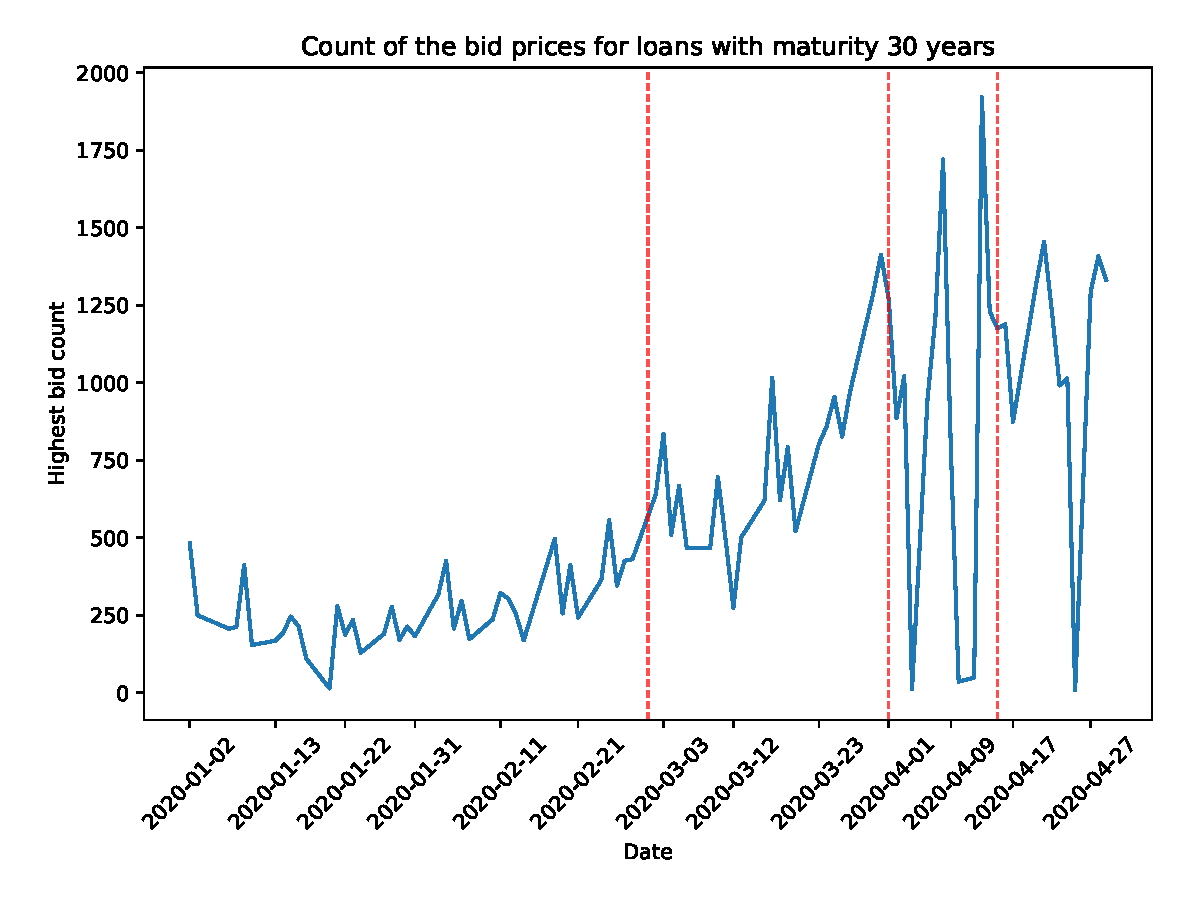
\includegraphics[width=0.998\textwidth]{../results/figures/winner_bid_count_mat30_loan1_timeseries_nr_3_3.75.pdf}
      \caption{ Number of auctions}
     \end{subfigure}
     \begin{subfigure}[b]{0.49\textwidth}
      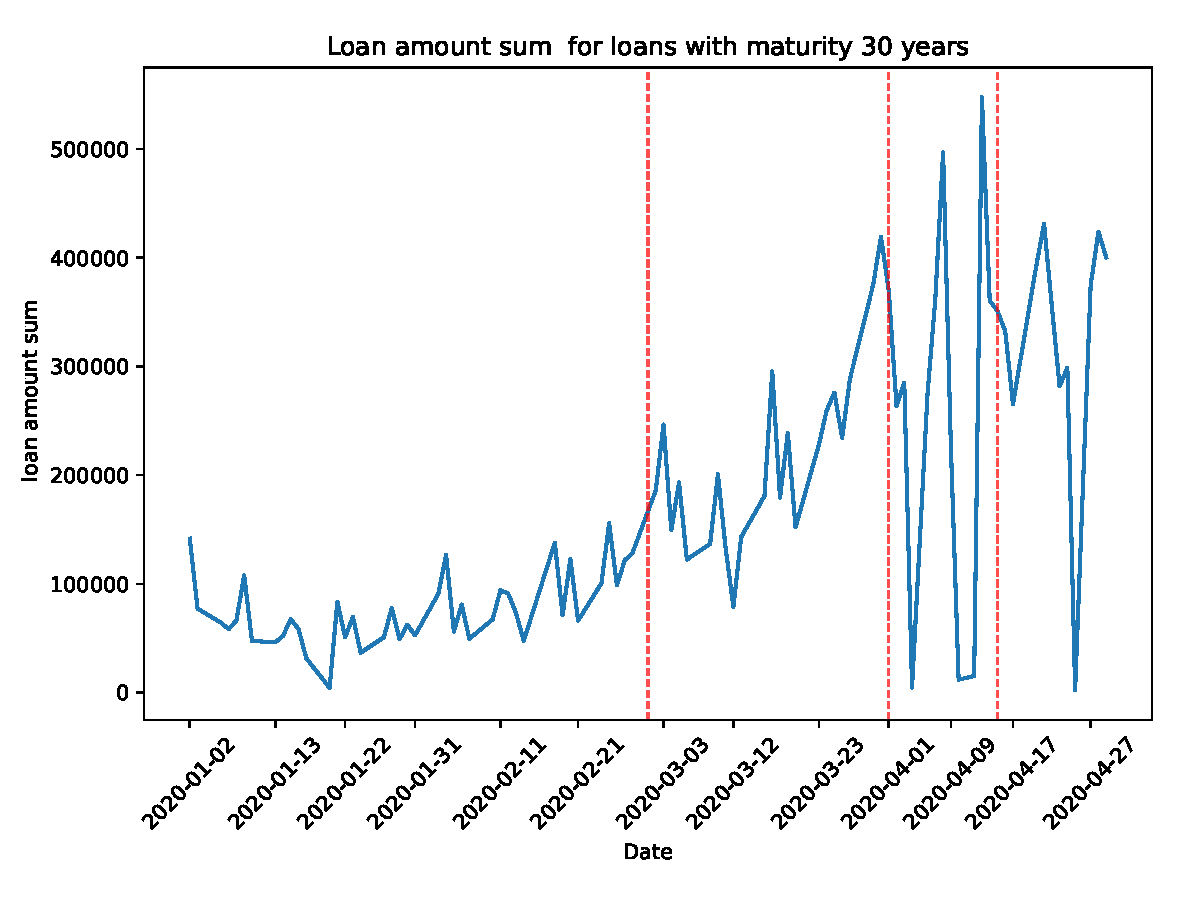
\includegraphics[width=0.998\textwidth]{../results/figures/LoanAmount_sum_mat30_loan1_timeseries_nr_3_3.75.pdf}
      \caption{ Daily loan amount}
     \end{subfigure}
     \begin{subfigure}[b]{0.49\textwidth}
      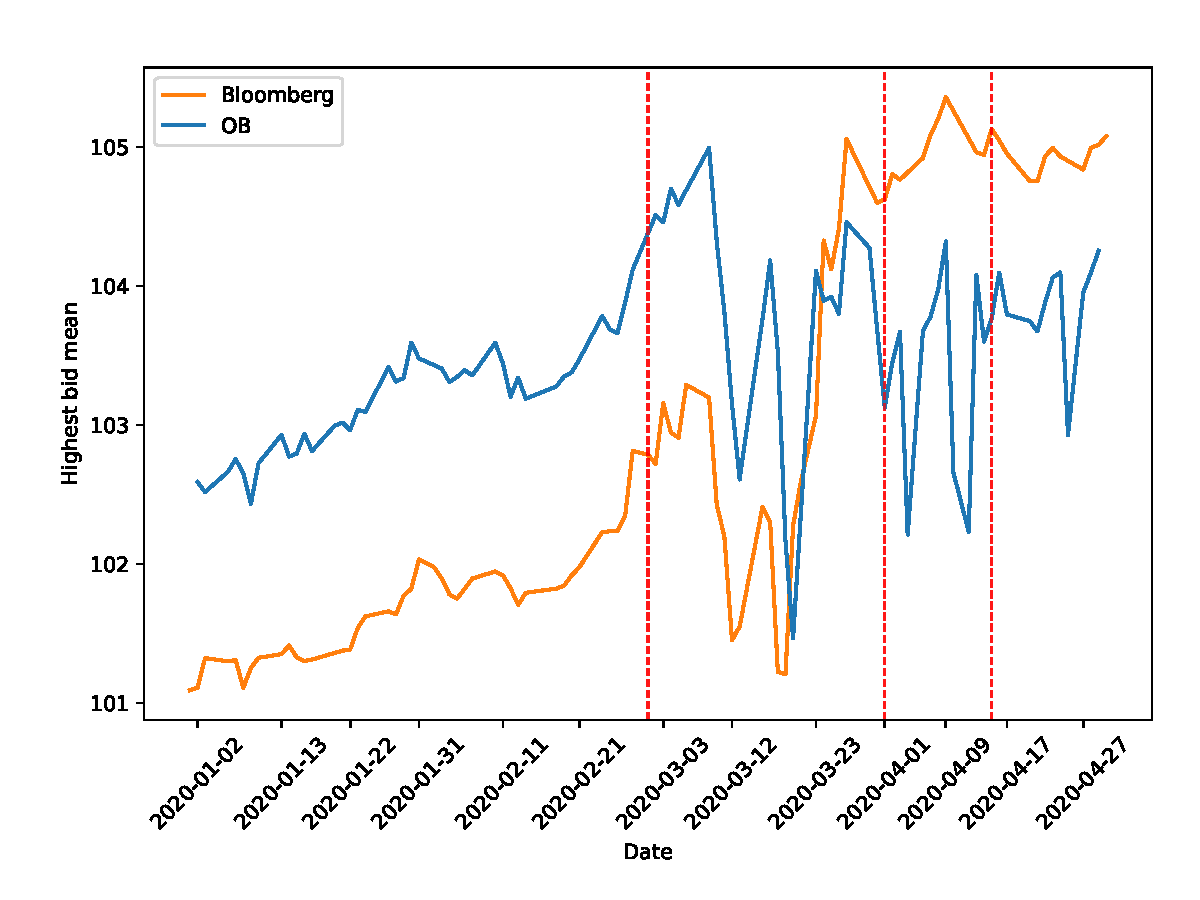
\includegraphics[width=0.998\textwidth]{../results/figures/w_winner_bid_mean_mat30_loan1_timeseries_nr_3_3.75.pdf}
      \caption{ Weighted mean of highest bid}
     \end{subfigure}
     \begin{subfigure}[b]{0.49\textwidth}
      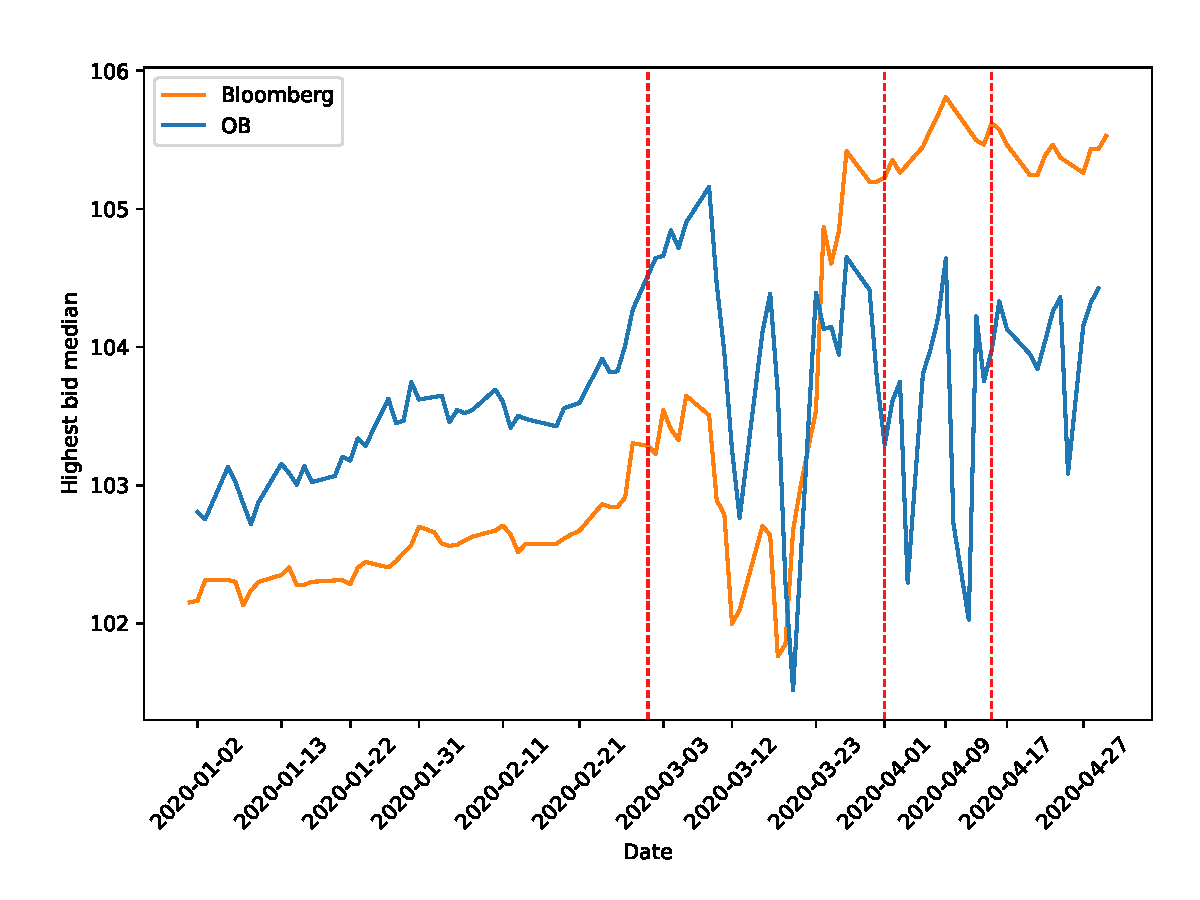
\includegraphics[width=0.998\textwidth]{../results/figures/winner_bid_median_mat30_loan1_timeseries_nr_3_3.75.pdf}
      \caption{ Median of highest bid}
     \end{subfigure}
   \caption{FED purchases of FNMA products in the early COVID period for note rate between 3\% and 3.75\%}
   \begin{minipage}{\textwidth}
      \footnotesize{\textit{Notes:} The figure shows the daily time series of auctios for Conforming loans 30 year maturity. The vertical lines are March 1, April 1st and April 15th. For reference, Bloomberg TBA prices are aggregated for all forward months and coupons between 2.5, 3 and 3.5. } 
      \end{minipage}
\end{figure}

\begin{figure}[h]
  \centering
  \begin{subfigure}[b]{0.49\textwidth}
      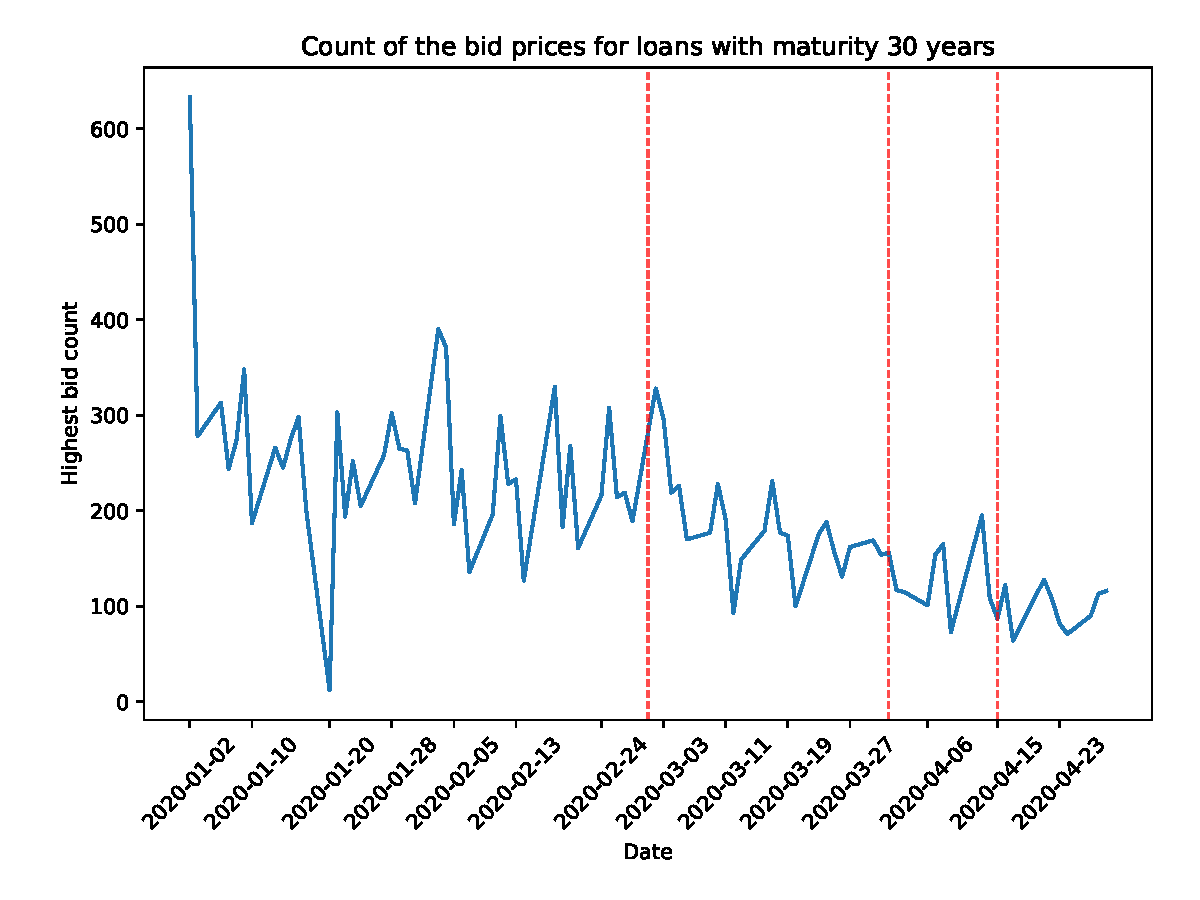
\includegraphics[width=0.998\textwidth]{../results/figures/winner_bid_count_mat30_loan1_timeseries_nr_4_4.75.pdf}
      \caption{ Number of auctions}
     \end{subfigure}
     \begin{subfigure}[b]{0.49\textwidth}
      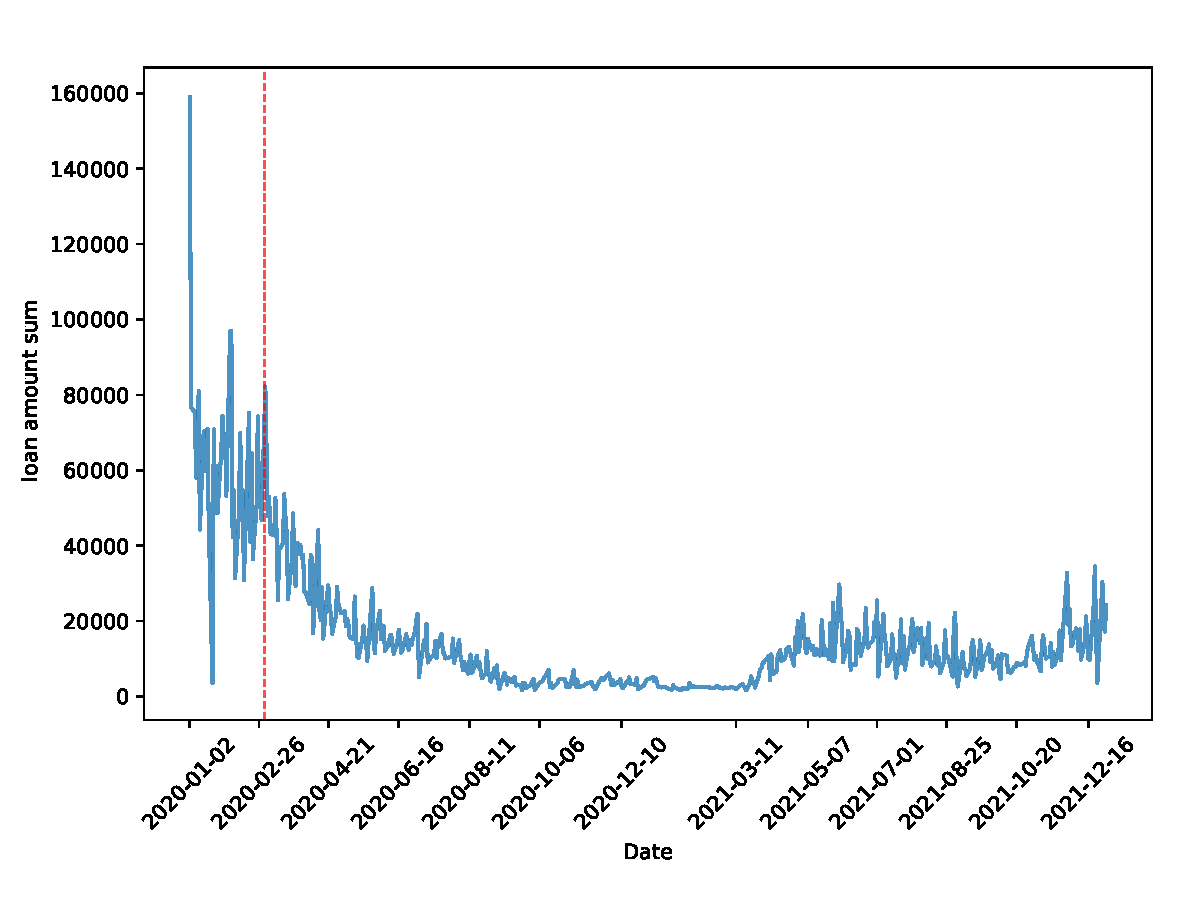
\includegraphics[width=0.998\textwidth]{../results/figures/LoanAmount_sum_mat30_loan1_timeseries_nr_4_4.75.pdf}
      \caption{ Daily loan amount}
     \end{subfigure}
     \begin{subfigure}[b]{0.49\textwidth}
      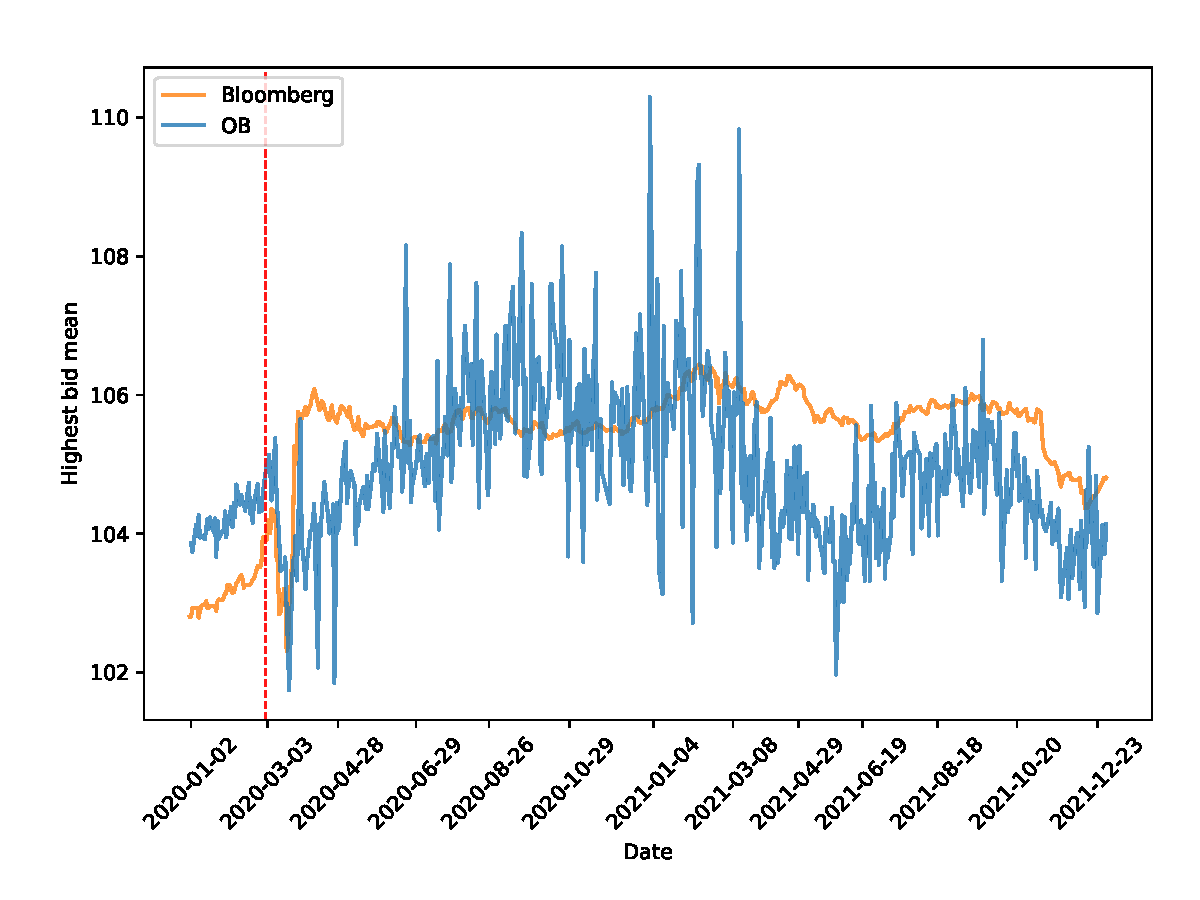
\includegraphics[width=0.998\textwidth]{../results/figures/w_winner_bid_mean_mat30_loan1_timeseries_nr_4_4.75.pdf}
      \caption{ Weighted mean of highest bid}
     \end{subfigure}
     \begin{subfigure}[b]{0.49\textwidth}
      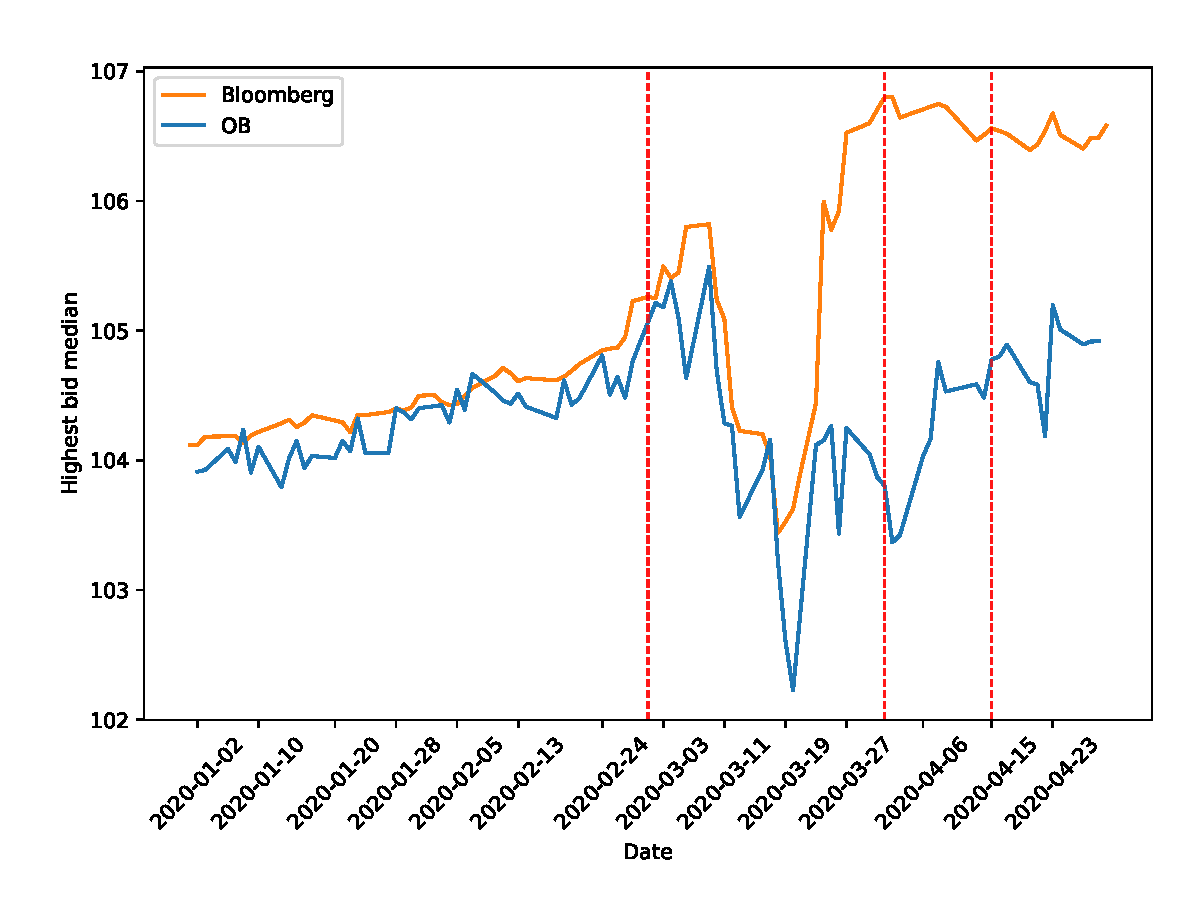
\includegraphics[width=0.998\textwidth]{../results/figures/winner_bid_median_mat30_loan1_timeseries_nr_4_4.75.pdf}
      \caption{ Median of highest bid}
     \end{subfigure}
   \caption{FED purchases of FNMA products in the early COVID period for note rate between 4\% and 4.75\%}
   \begin{minipage}{\textwidth}
      \footnotesize{\textit{Notes:} The figure shows the daily time series of auctios for Conforming loans 30 year maturity. The vertical lines are March 1, April 1st and April 15th. For reference, Bloomberg TBA prices are aggregated for all forward months and coupons 3.5, 4 and 4.5. } 
      \end{minipage}
\end{figure}

\pagebreak

\subsection{Auction characteristics}



\end{document}
